\chapter{Model Examination}
\label{chapt:VALIDATION}
The models created in  \S\ref{chapt:ALGORITHM} were then examined and assessed. As an unsupervised learning algorithm, it is difficult to assess model quality, due to a lack of concrete metrics to comparisons\footnote{This is to say, there is no objective `similarity' relationship value between two words.}. The Word2Vec development team tested models against $\sim$ 10,000 semantic and syntactic relationships (See Figure \ref{fig:KINGQUEEN})\cite{word2vec1} \cite{word2vec2} \cite{word2veckingqueen}. The scope of this project does not extend to such elaborate tests. In the section, some examples of model strengths are given and techniques for using word vectors and visualisation are presented. 
\section{Word Similarities}
Word similarities can be be obtained by direct comparison of their word vectors. For words $\alpha$ and $\beta$, with vectors $\mathbf{\nu^\alpha}$ and $\mathbf{\nu^\beta}$.  A possible metric is to compute euclidean distance between $\mathbf{\nu^\alpha}$ and $\mathbf{\nu^\beta}$, 

$$S_{euclid} = \sqrt{\sum_{i=1}^{D}(\nu_i^{\alpha}-\nu_i^{\beta})^{2}} $$

where $D$ is the dimensionality ($D$=100). This metric simply describes the distance between the end points of $\mathbf{\nu^\alpha}$ and $\mathbf{\nu^\beta}$. A larger $S_{euclid}$ indicates weaker similarity. A second similarity metric is the \emph{cosine similarity}, a measure of the directionality of $\mathbf{\nu^\alpha}$ and $\mathbf{\nu^\beta}$. A value close to 1 corresponds to high similarity of $\alpha$ and $\beta$. Cosine similarity is computed as:
$$S_{cos}=\frac{\mathbf{\nu^\alpha} \cdot \mathbf{\nu^\beta}}{|\mathbf{\nu^\alpha}| |\mathbf{\nu^\beta}|} = \frac{\displaystyle\sum_{i=1}^{D} \nu^{(\alpha)}_{i}\nu^{(\beta)}_{i}}{\left(\displaystyle\sum_{i=1}^{D} (\nu^{(\alpha)}_{i})^2\right)^{1/2} \left(\displaystyle\sum_{i=1}^{D} (\nu^{(\beta)}_{i})^2\right)^{1/2}}
$$
The CBOW and skip-gram models were examined using these metrics. For a given word, they were requested to return the three words in the corpus with highest similarity. Some examples are given in tables \ref{tab:COSINESIMS} and \ref{tab:EUCLIDSIMS}.
\begin{table}[H]
\begin{center}
\caption[Word similarity examinations with cosine similarity]{Closest words to test words using cosine similarity}
\label{tab:COSINESIMS}
\begin{tabular}{||c||c|c|c|c||}
\hline
Model     & Test Word              & Most Similar & 2nd & 3rd \\ \hhline{||=||=|=|=|=||}
CBOW      & \multirow{2}{*}{Iron} & Chromium             &  Manganes   &   Nickel  \\ \cline{1-1} \cline{3-5} 
Skip-gram &                   &  Chromium            &   Manganes  &  Nickel   \\ 
\hhline{||=||=|=|=|=||}
CBOW      & \multirow{2}{*}{Colloid} & Nanoparticl             &  Nanos   &   Monodispers  \\ \cline{1-1} \cline{3-5} 
Skip-gram &                   &  Particl            &   Spheric  &  Suspens   \\ 
\hhline{||=||=|=|=|=||}
CBOW      & \multirow{2}{*}{Statistical} & Varianc             &  Bayesian   &   Multivari  \\ \cline{1-1} \cline{3-5} 
Skip-gram &                   &  Nonparametr            &   Varianc  &  Bootstrap   \\ 
\hhline{||=||=|=|=|=||}
CBOW      & \multirow{2}{*}{Plastic} & Thermoplast             &  Elastomer   & Nonwoven    \\ \cline{1-1} \cline{3-5} 
Skip-gram &                   &  Nonwoven            &   Thermoplast  &  Textolit   \\ 
\hhline{||=||=|=|=|=||}
CBOW      & \multirow{2}{*}{Catalyst} & Cocatalyst             &  Nanocatalyst   & Precatalyst    \\ \cline{1-1} \cline{3-5} 
Skip-gram &                   &  Catalyt            &   Nanocatalyst  &  Polystyrylbipyridin   \\ 
\hhline{||=||=|=|=|=||}
\end{tabular}
\end{center}
\end{table}

\begin{table}[h!]
\begin{center}
\caption[Word similarity examinations with euclidean similarity]{Closest words to test words using Euclidean similarity}
\label{tab:EUCLIDSIMS}
\begin{tabular}{||c||c|c|c|c||}
\hline
Model     & Test Word              & Most Similar & 2nd & 3rd \\ \hhline{||=||=|=|=|=||}
CBOW      & \multirow{2}{*}{Iron} & Chromium             &  Managanes   &   Nickel  \\ \cline{1-1} \cline{3-5} 
Skip-gram &                   &  Chromium            &   Manganes  &  Nickel   \\ 
\hhline{||=||=|=|=|=||}
CBOW      & \multirow{2}{*}{Colloid} & Nanos             &  Ultrafin   &   Agglomer  \\ \cline{1-1} \cline{3-5} 
Skip-gram &                   &  Particl            &   Suspens  &  Spheric   \\ 
\hhline{||=||=|=|=|=||}
CBOW      & \multirow{2}{*}{Statistical} & Varianc             &  Phenomenolog   &   Bayesian  \\ \cline{1-1} \cline{3-5} 
Skip-gram &                   &  Nonparametr            &   Bivari  &  Multigrid   \\ 
\hhline{||=||=|=|=|=||}
CBOW      & \multirow{2}{*}{Plastic} & Thermoplast             &  Elastomer   & Mold    \\ \cline{1-1} \cline{3-5} 
Skip-gram &                   &  NRL            &   Prepreg  &  Sealant   \\ 
\hhline{||=||=|=|=|=||}
CBOW      & \multirow{2}{*}{Catalyst} & Nanocatalyst             &  Cocatalyst   & Precatalyst    \\ \cline{1-1} \cline{3-5} 
Skip-gram &                   &  Catalyt            &   Molybdena  &  Nimo   \\ 
\hhline{||=||=|=|=|=||}
\end{tabular}
\end{center}
\end{table}
As shown above, the models perform well, returning intuitively similar words to the test word.\footnote{Note that returned words are 'stemmed' from use of stemming algorithm before training. It is not difficult to interpret derived words from their stems}. In most cases, chemical inference is represented in some way (e.g. the models understood that catalysts and nanocatalysts are closely-connected concepts).

It was observed that the skip-gram model gave misleading positives more frequently. \footnote{in the catalyst case above, skip-gram associated a stemming false negative and gave a specific catalysed compound to the `catalyst' test word than more obvious, fundamental associations}. The CBOW model was considered to be superior for word-word comparisons. It was also noted that CBOW had stronger agreement between euclidean and cosine similarity metrics, however, euclidean similarity gave poorer general perform.\footnote{`NRL' in the `Plastic' category of skip-gram is a typical example of poorer euclidean performance. NRL appears to be a reference to the Navy Reseach Laboratory. }. It is noted that cosine similarity is the accepted similarity metric in the literature \cite{word2vec1} \cite{word2vec2} \cite{doc2vec}.

\section{Document Similarities}
The models detailed in \S\ref{chapt:ALGORITHM} were then tested for document vector similarity. A document was chosen from the corpus, the three most similar articles were computed for each model and results assessed. One test document was \texttt{DOI: 10.1134/s0036024412120266} \cite{docassay}, the title:


\texttt{`Photochemical transformations of anthraquinone in polymeric alcohols'}.

 The TF-IDF models (CBOW-TFIDF-S, CBOW-TFIDF-W, SG-TFIDF-S, SG-TFIDF-W) suffered from mathematical conditioning problems, and gave poor predictions. The remaining models' most similar documents \footnote{Cosine similarity was used, as it performed better than euclidean similarity for document vectors.} for this test document are shown in table \ref{tab:DOCSIMS}:
\begin{table}[H]
\centering
\caption[Examination of Document Vector similarities]{Document Vector Similarities to \cite {docassay}}
\label{tab:DOCSIMS}
\begin{tabular}{|l|p{2cm}|p{4cm}|p{2cm}|p{4cm}|}
\hline
Model           & DOI            & Title            & DOI              & Title              \\ \hline
CBOW-W               & 10.1080/ 00222338 208074396         & \footnotesize{Oxidation of Poly(dimethylbutadiene) Popcorn Polymer} &  10.1246/ cl.1974.133               &                   \footnotesize{photochemical reaction of 2-cyanoquinoline 1-oxides in an acidic alcohol. synthesis of 6-alkoxy-2-cyanoquinolines} \\ \hline
CBOW-S               & 10.1002/ pol.1985 .170230401          &  \footnotesize{Polymerization of glycidol and its derivatives: A new rearrangement polymerization}
                & 10.1080/ 002223381 08074381                & \footnotesize{Cyclic Acetal-Photosensitized Polymerization. 9. Photopolymerization of Triallylidene Sorbitol}
                   \\ \hline
SG-S                 & 10.1002/ pola.1991. 080290207            &   \footnotesize{Photochemical synthesis of nitroxyl free radicals in the presence of vinyl monomers}
               &  10.1002/ pola.10311              &  \footnotesize{Benzyl alcohols as accelerators in the photoinitiated cationic polymerization of epoxide monomers}
                  \\ \hline
SG-W                 & 10.1080/ 00222338 208074396            &    \footnotesize{Oxidation of Poly(dimethylbutadiene) Popcorn Polymer}
              & 10.1080/ 00222338 408077237                &  \footnotesize{Photopolymerization of Acrylonitrile: Benzophenone-Isopropanol System as Initiator}
                 \\ \hline
doc2vec                    &  10.1002/ pola.10059              &  \footnotesize{Aqueous photopolymerization with visible-light photoinitiators: Acrylamide polymerization photoinitiated with a phenoxazine dye/amine system}
                & 10.1080/ 10587259 408029732                 & \footnotesize{ An Investigation into the Solid-State Behaviour of Anthraquinone and Its Derivatives}
                 \\ \hline
\end{tabular}
\end{table}
The document vectors generated by the Doc2Vec model had considerably better performance, and thus were taken forward as the model of choice for further analysis.  
\section{Visualisation Techniques}
\subsection{Network Visualisation}
High Dimensional systems are hard to visualise but there are several methods available to visualise high-dimensional data. PCA\footnote{Principle Component Analysis}\cite{PCA}, a well-established technique reduces dimensionality by a series of orthogonal transformations. T-SNE\footnote{t-distributed stochastic network embedding }, a state of the art technique to reduce dimensionality by preserving spatial clusters of vectors at high dimensions \cite{TSNE}. These techniques allows 100-dimensional document vectors to be collapsed to points on an arbitrary 2D plane, to give a visualised `snapshot' of the semantic space. 
Figures \ref{fig:PCA_snap} and \ref{fig:TSNE_snap} show PCA and TSNE reductions\footnote{performed using scikitlearn and python} on 10,000 document vectors randomly selected from the Doc2Vec model representation of \Delta6. \cite{scikitlearn}.

\begin{figure}[H]
  \centering
  \begin{minipage}[b]{0.49\textwidth}
	\begin{center}\textbf{PCA Dimensional Reduction}\end{center}
    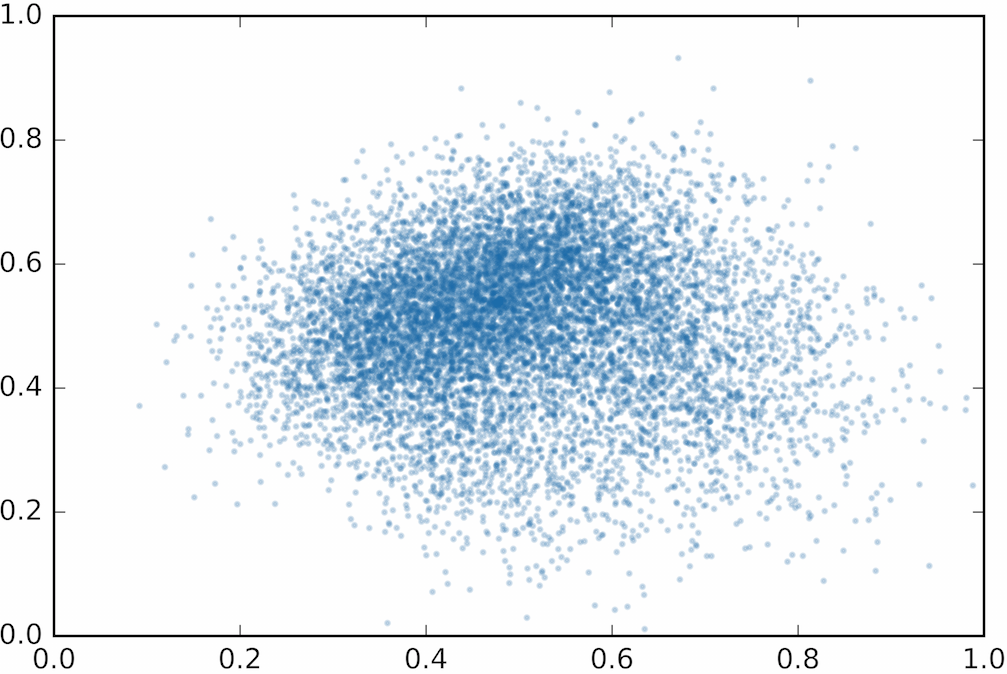
\includegraphics[width=\textwidth]{Validation/pca2.png}
    \caption[PCA Dimensional Reduction]{PCA map of 10,000 documents in the corpus. PCA has not any particular structure. The dimensional reduction task is probably too difficult for PCA.}
      \label{fig:PCA_snap}
  \end{minipage}
  \hfill
  \begin{minipage}[b]{0.49\textwidth}
  \begin{center}\textbf{TSNE Dimensional Reduction}\end{center}
    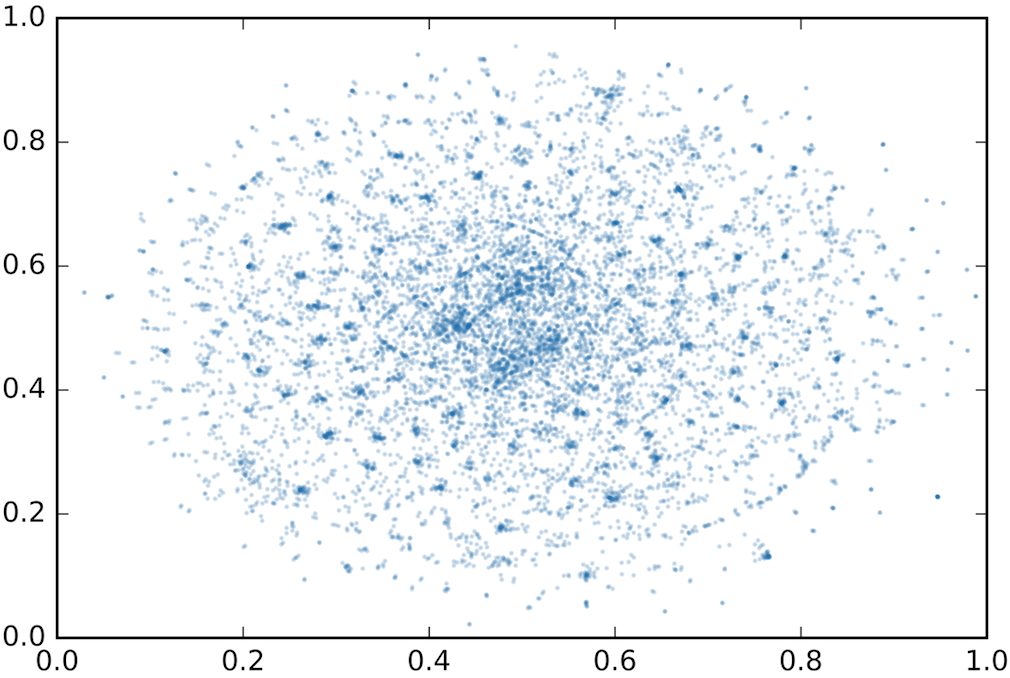
\includegraphics[width=\textwidth]{Validation/tsne2.png}
    \caption[TSNE Dimensional Reduction]{TSNE map of the same 10,000 documents. Document vectors have gathered into noticeable clusters, with non negligible outlier documents between clusters. }
      \label{fig:TSNE_snap}

  \end{minipage}
\end{figure}
The PCA reduction shows a dark central area, suggesting most vectors are `smeared' about a common direction. The map is not entirely symmetric which is what would be expected for random vectors. It was expected that document vectors would be distributed into clusters representing particular research fields within the literature. This is borne out by the TSNE reduction, which has resolved many clusters. There is a significant portion of document vectors scattered between dark cluster spots, which may be could interpreted as `interdisciplinary'.
TSNE is based upon euclidean distance, which is noted not to be the best similarity measure so, whilst qualitatively useful, TSNE maps were interpreted cautiously.
\subsection{Networks and Network Visualisation}
\label{sec:COSINEMAT}
A similarity matrix $\mathbf{C}$ was defined between a sets of documents. For a set of documents  A (with $a$ documents) and B (with $b$ documents) define document matrices of document vectors $\mathbf{A}$ and $\mathbf{B}$ such that 

$$\mathbf{A} = \left( \begin{array}{cccc}
\vdots & \vdots & \vdots & \vdots \\
\mathbf{w}_1 & \mathbf{w}_1 & \cdots & \mathbf{w}_a \\
\vdots & \vdots & \vdots & \vdots \\ \end{array} \right) , \mathbf{B} = \left( \begin{array}{cccc}
\vdots & \vdots & \vdots & \vdots \\
\mathbf{v}_1 & \mathbf{v}_1 & \cdots & \mathbf{v}_b \\
\vdots & \vdots & \vdots & \vdots \\ \end{array} \right)$$ where $w$ and $v$ are document vectors.
The cosine matrix $\mathbf{C}$ is then defined as $\mathbf{C}_{i , j} = cosine \left(\theta_{i , j} \right)$ where element i j contains the cosine between $i$th document vector in A and $j$th document vector in B:
$$\mathbf{C}=\mathbf{A}^T \mathbf{B} \oslash \left( diag(\mathbf{A}^T \mathbf{A})^T diag(\mathbf{B}^T \mathbf{B}) \right)^{\circ\frac12}$$
where $\oslash$ and $^{\circ\frac12}$ indicate Hadamard division and Hadamard square root \footnote{Elementwise division and Elementwise square root}, $diag(Q)$ the $1 \times n$ matrix formed from the diagonal of matrix $Q$. This matrix represents a network where each document in A is a node with an edge to every document in B with a weight equal to the cosine. If A is B, then the matrix is a fully connected network\footnote{That is to say, every document node has an edge to every other document in the set}. This network can be visualised using specialist software\footnote{Gephi, a powerful, open source network visualisation and analysis suite, was used for this purpose. } \cite{gephi}. Figure \ref{fig:gephi_exp} visualises the same 10,000 document sample as a network graph.
\begin{center}
\begin{figure}[H]
  \centering
  \textbf{Network Visualisation of 10,000 document sample}
     \makebox[\textwidth][c]{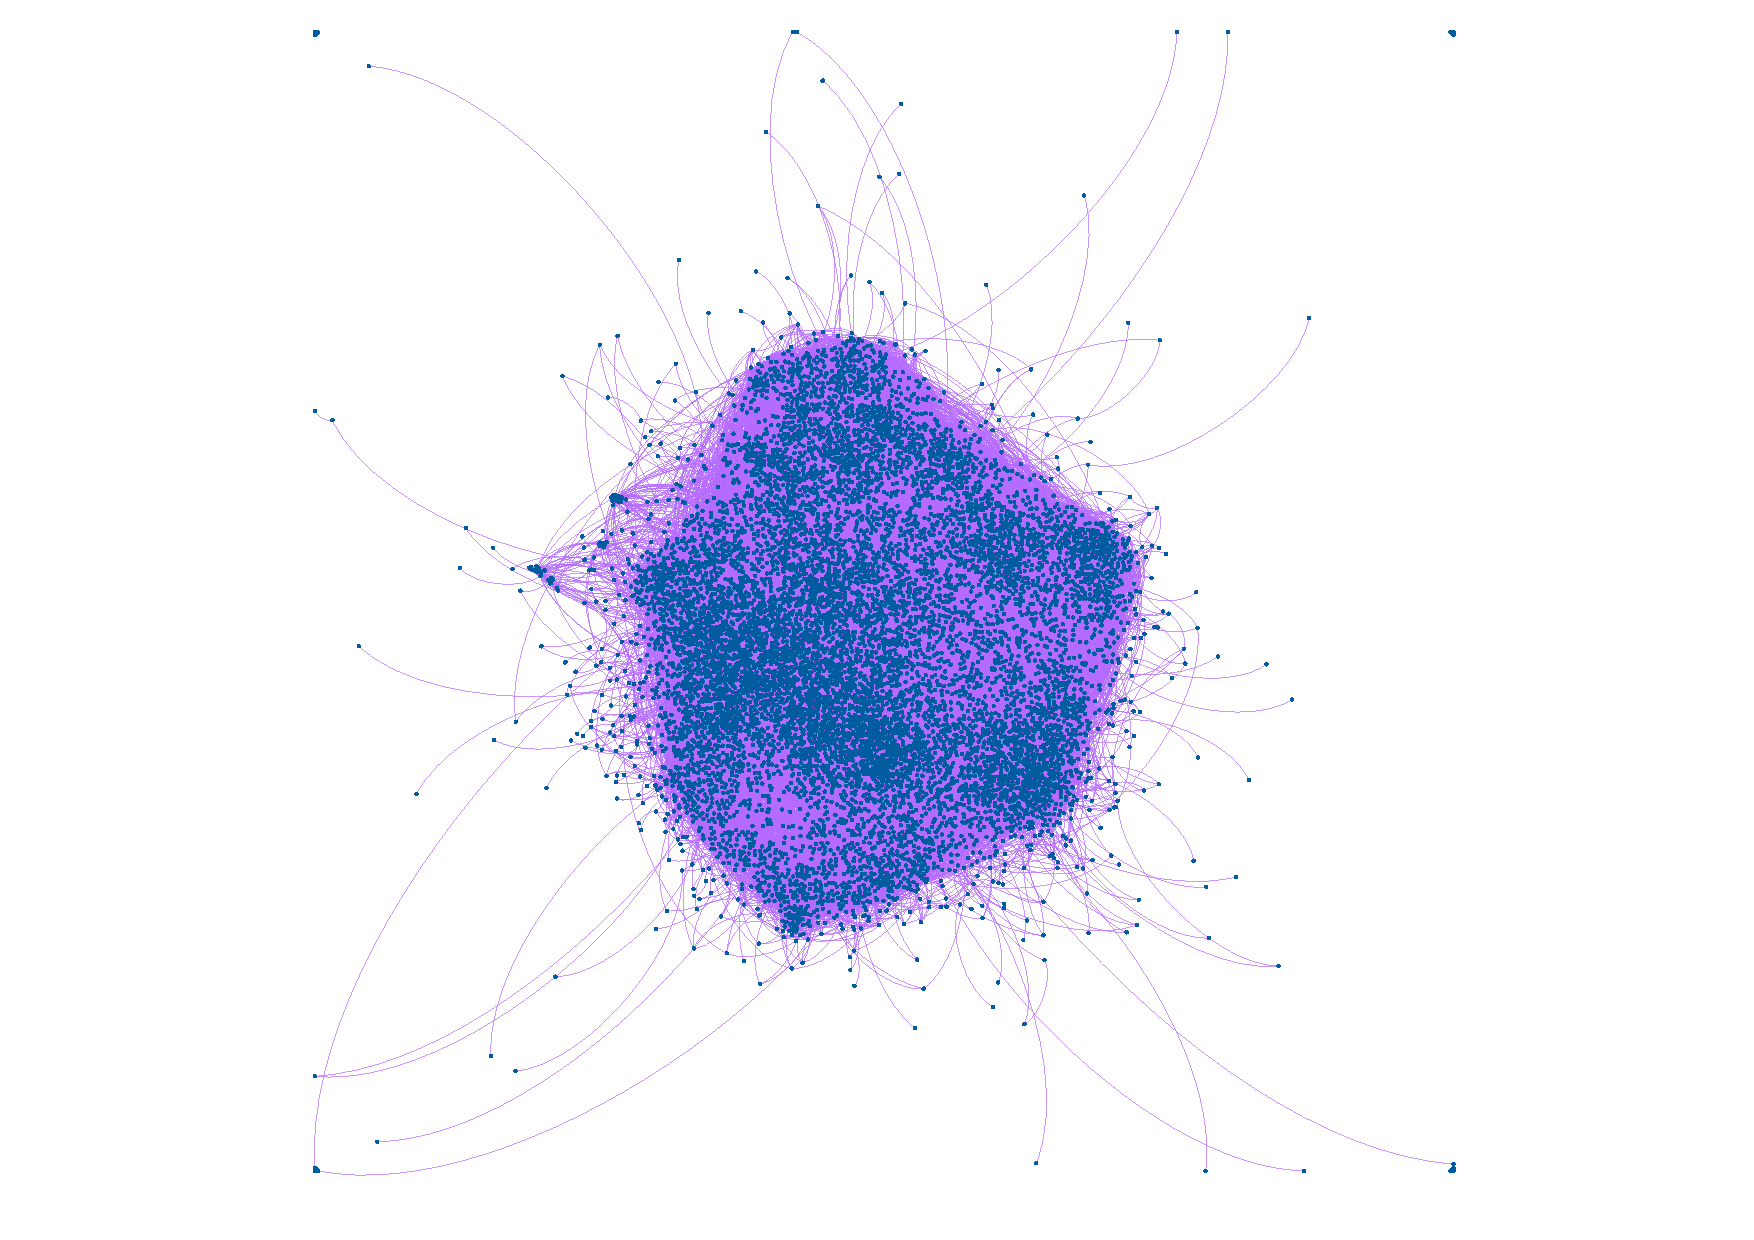
\includegraphics[width=1.2\textwidth]{Validation/sample.pdf}}
    \caption[Network Visualisation of 10,000 document random sample]{A Network visualisation of the 10,000 document sample. Nodes (blue) are spatially distributed by modelling the edges (purple) as springs connecting nodes with spring constants equal to cosine similarity, then allowing the system to approach equilibrium. Edges were only placed between nodes with cosine similarity greater than 0.35 for computational tractability. The edges have been curved to aid visualisation.}
    \label{fig:gephi_exp}

\end{figure} 
\end{center}
It can be seen that concentrations of documents also form in the network visualisation. There are noticeable outlier documents far from the central clusters \footnote{These articles are predicted to be short, or qualitatively different from, the majority, e.g. addenda or retraction notices, rather than proper articles.}. Also note that the network visualisation technique is dependent only on cosine similarity, so was considered a more reliable analytical tool than TSNE. Treating the system as a network graph also enables powerful network analytic algorithms to be applied.